\chapter{Construction} \label{chptr:construction}

The first step in screening using locating arrays is to construct the locating array.
In this step, one chooses $k$ factors $F_1, F_2, \dots, F_k$, to be used in screening and determines the number of levels $\ell_j$ for each factor $F_j$, and then constructs a valid locating array.
Producing any locating array is trivial.
A full-factorial screening experiment is a locating array since every possible combination of level-to-factor assignments exists in the design.
However, we focus on cases where many possible factors have been chosen for screening.
In such cases, the size of a full-factorial experiment is extremely large.
The large system introduced in Section \ref{sect:rel_analysis} with $k = 100$, for example, contains over $10^{69}$ tests if a full-factorial experiment were to be used.
Such sizes are infeasible, and this chapter discusses strategies to construct locating arrays that are more useful in practice.

\section{Desirable Properties} \label{sect:properties}

Certain desirable properties exist when considering the construction of locating arrays along with their usages.
First, it is desirable for locating arrays to have few rows (or tests).
Because every test takes some amount of time to complete, locating arrays with billions of rows are undesirable and likely impossible to use.
However, "few" is a relative attribute, and this property is therefore strongly dependent on how practical it is to run multiple tests in a particular environment.
Second, it is desirable for locating arrays to produce accurate results when they are used.
This second property is intuitive, but it is not completely clear what types of locating arrays produce accurate results.
We hypothesize that locating arrays can be constructed to produce more accurate results through the use of a particular attribute that we refer to as {\em separation}.
We first motivate separation with an example and then formally define it.

Suppose we construct a locating array with hundreds of rows.
Next, we construct the associated compressive sensing matrix, but observe that two of its columns are quite similar and differ in only a single row.
If we then attempt to use this compressive sensing matrix to produce accurate results, the two similar columns are likely (almost) indistinguishable.
Furthermore, if the term corresponding to one column is truly significant while the term corresponding to the other column is insignificant, then it is likely difficult to determine which of the two is the important term (and which to discard).
Finally, if an error in measurement occurs in the unique test where the two columns differ, then the locating property of the array is lost entirely.
Therefore, we hypothesize that it is beneficial for every column in the compressive sensing matrix to differ from every other column in at least $\delta$ rows.
In this case, we refer to the associated locating array as exhibiting separation $\delta$.

A formal definition of separation $\delta$ is the minimum difference between any two columns of an associated compressive sensing matrix in the number of rows where the columns differ.
Thus it is the number of rows in which any two terms are guaranteed to differ for a particular locating array.
If a locating array, $A$, exhibits separation $\delta$, then for every two terms $T_1$, $T_2$ where $T_1 \neq T_2$, we have that $|(\rho(A,T_1) \cup \rho(A,T_2)) \setminus (\rho(A,T_1) \cap \rho(A,T_2))| \geq \delta$.

For example, Table \ref{tab:la_delta2} shows a locating array for factors $F_1, F_2$ both with levels $v_1, v_2, v_3$, followed by three columns from the corresponding compressive sensing matrix.
In this example we focus on only these three columns for simplicity and do not show the remainder of the compressive sensing matrix.
Three unique pairs of columns exist from the three compressive sensing columns shown.
The first pair is columns one and two, and this pair of columns differs in four rows (5, 12, 13, and 16).
The second pair is columns one and three, and this pair of columns differs in two rows (5 and 12).
The third pair is columns two and three, and this pair of columns differs in two rows (13 and 16).
The minimum difference between these three pairs is two rows, and the locating array in Table \ref{tab:la_delta2} therefore exhibits separation $\delta=2$.

\begin{center}
\begin{table}[htbp]
\caption{Separation Example - $\delta = 2$}
\label{tab:la_delta2}
\begin{tabularx}{\textwidth}{|1|3|6|}
\hline
\multicolumn{3}{|c|}{Locating Array} \\
\hline
Test & $F_1$ & $F_2$ \\
\hline
 1 & $v_1$ & $v_3$ \\
 2 & $v_2$ & $v_2$ \\
 3 & $v_2$ & $v_3$ \\
 4 & $v_3$ & $v_3$ \\
 5 & $v_3$ & $v_1$ \\
 6 & $v_1$ & $v_3$ \\
 7 & $v_3$ & $v_2$ \\
 8 & $v_3$ & $v_2$ \\
 9 & $v_1$ & $v_2$ \\
10 & $v_2$ & $v_2$ \\
11 & $v_2$ & $v_3$ \\
12 & $v_3$ & $v_1$ \\
13 & $v_2$ & $v_1$ \\
14 & $v_3$ & $v_3$ \\
15 & $v_1$ & $v_2$ \\
16 & $v_2$ & $v_1$ \\
\hline
\end{tabularx}

\begin{tabularx}{\textwidth}{|1|3|3|3|}
\hline
\multicolumn{4}{|c|}{Partial Compressive Sensing Matrix} \\
\hline
Test & $F_2 = v_1$ & $F_2 = v_1$ \& $F_1 = v_1$ & $F_2 = v_1$ \& $F_1 = v_2$ \\
\hline
 1 & -1	& -1	& -1 \\
 2 & -1	& -1	& -1 \\
 3 & -1	& -1	& -1 \\
 4 & -1	& -1	& -1 \\
 5 & 1	& -1	& -1 \\
 6 & -1	& -1	& -1 \\
 7 & -1	& -1	& -1 \\
 8 & -1	& -1	& -1 \\
 9 & -1	& -1	& -1 \\
10 & -1	& -1	& -1 \\
11 & -1	& -1	& -1 \\
12 & 1	& -1	& -1 \\
13 & 1	& -1	& 1  \\
14 & -1	& -1	& -1 \\
15 & -1	& -1	& -1 \\
16 & 1	& -1	& 1  \\
\hline
\end{tabularx}

\end{table}
\end{center}

Table \ref{tab:la_delta3} continues the example in Table \ref{tab:la_delta2} by adding another row to the locating array (and compressive sensing matrix).
The second and third pairs both differ in the additional test.
The minimum difference between the pairs is now 3 rows and the separation of this locating array is $\delta=3$.

\begin{center}
\begin{table}[htbp]
\caption{Separation Example Continued - $\delta = 3$}
\label{tab:la_delta3}
\begin{tabularx}{\textwidth}{|2|4|4|}
\hline
\multicolumn{3}{|c|}{Locating Array} \\
\hline
Test & $F_1$ & $F_2$ \\
\hline
17 & $v_1$ & $v_1$ \\
\hline
\end{tabularx}

\begin{tabularx}{\textwidth}{|1|3|3|3|}
\hline
\multicolumn{4}{|c|}{Partial Compressive Sensing Matrix} \\
\hline
Test & $F_2 = v_1$ & $F_2 = v_1$ \& $F_1 = v_1$ & $F_2 = v_1$ \& $F_1 = v_2$ \\
\hline
17 & 1	& 1	& -1 \\
\hline
\end{tabularx}

\end{table}
\end{center}

Finally, we repeat the test added in Table \ref{tab:la_delta3} to continue the separation example in Table \ref{tab:la_delta4}.
The second and third pairs both differ again in the additional test.
The minimum difference between the pairs is now 4 rows and the separation of this locating array is $\delta=4$.
This example shows how strategically adding rows to a locating array can increase its separation.

\begin{center}
\begin{table}[htbp]
\caption{Separation Example Continued - $\delta = 4$}
\label{tab:la_delta4}
\begin{tabularx}{\textwidth}{|2|4|4|}
\hline
\multicolumn{3}{|c|}{Locating Array} \\
\hline
Test & $F_1$ & $F_2$ \\
\hline
18 & $v_1$ & $v_1$ \\
\hline
\end{tabularx}

\begin{tabularx}{\textwidth}{|1|3|3|3|}
\hline
\multicolumn{4}{|c|}{Partial Compressive Sensing Matrix} \\
\hline
Test & $F_2 = v_1$ & $F_2 = v_1$ \& $F_1 = v_1$ & $F_2 = v_1$ \& $F_1 = v_2$ \\
\hline
18 & 1	& 1	& -1 \\
\hline
\end{tabularx}

\end{table}
\end{center}

Note that an array must have separation of at least one to satisfy the locating property.
However, we hypothesize that when locating arrays exhibit higher separation, they produce more accurate results when used.
Evidence supporting this hypothesis is presented in Section \ref{sect:separation}.

\section{Initial Greedy Approach} \label{sect:greedy}

A greedy approach can be used to quickly create a simple locating array without extra separation.
This approach begins with any array of tests, $A$, that does not have the locating property (it can be empty), and adds rows in a greedy fashion until the locating property is satisfied.
This greedy fashion of adding rows relies on a score indicating how close $A$ is to having the locating property.
One possible, and effective, way to achieve this scoring, is to count the unique pairs of identical columns in the compressive sensing matrix, $M$, for $A$.
This scoring approach yields a lower score when $A$ improves and is closer to having the locating property.

Suppose that $A$ is an empty array.
Then all columns in $M$ are also empty and are therefore all identical.
Any combination of two columns in $M$ is a pair of identical columns, and there are then $m \choose 2$ unique pairs of identical columns where $m$ is the number of columns in $M$.
It is not possible for the number of identical columns in $M$ to be more than $m \choose 2$ so this is the largest possible score for $A$.
Intuitively, an empty array is as far as possible from having the locating property and therefore exhibits the maximum score.

Suppose now that $A$ is a valid locating array.
Then not a single pair of identical columns exists in $M$ because the locating property is satisfied, and the score of $A$ is $0$, the minimum score.
Therefore, the score simply counts the deficiencies in $A$, and once the score is $0$, $A$ has no deficiencies and construction is complete.

Algorithm \ref{alg:greedy_construction} lists the detailed steps of this greedy approach.
The algorithm begins with an empty array, $A$, with 0 rows and then adds rows until $A$ is a locating array.
It is important to note that adding any row to $A$ cannot worsen its score (adding a row cannot create more unique pairs of duplicate columns in the compressive sensing matrix).
First, a row of random factor assignments corresponding to the $\mathit{factors}$ parameter is generated and added to $A$.
The entries of this row are origininally marked as not \textit{finalized} which means they can still be changed to improve the score of the locating array.
All pairs of duplicate columns in the compressive sensing matrix are then found, and all columns included in these pairs are iterated through.
For each column, the algorithm attempts to update and finalize the factor assignments affecting this column so that the column entry in the most recently added row changes, and the column is no longer part of a duplicate pair.
This update is the crux of the algorithm, and only occurs if the affecting factor assignments have not yet been marked as finalized.
The score of $A$ is checked after the update and then the array is reverted to its previous state.
After all columns have been checked, the algorithm keeps the column updates that produced the best score improvement in $A$.
The most recently added row now contains factor assignments that are marked as finalized and these assignments can no longer change.
The algorithm then repeats the process of checking all pairs of duplicate columns until the score cannot be further improved.
Finally, another row is added and the entire process repeats until the array contains no deficiencies and is a valid locating array.

\begin{algorithm}[pthb]
\caption{$\mathrm{Greedy\_Construction}(\mathit{factors})$}
\label{alg:greedy_construction}

\begin{algorithmic}[1]
\REQUIRE List of factors (including their levels)
\ENSURE A valid locating array
\STATE $A \gets$ [empty array with 0 rows]
\WHILE{$A.getScore() > 0$}
	\STATE $row \gets$ [random row of valid factor assignments for $factors$]
	\FOR{$assignment \in row$}
		\STATE $assignment.finalized \gets False$
	\ENDFOR
	\STATE {Add $row$ to $A$, and keep $row$ as reference}
	\WHILE{$True$}
		\STATE $M \gets createCSM(A)$
		\STATE $dPairs \gets$ [all pairs of duplicate columns in $M$]
		\STATE $bestA \gets A$
		\FOR{$pair \in dPairs$} \label{line:time_bound}
			\FOR{$column \in pair.columns$}
				\STATE $Acopy \gets$ [copy of $A$]
				\FOR{$factor \in column.factors$}
					\STATE $assignment \gets row.assignments(factor)$
					\IF{NOT $assignment.finalized$}
						\STATE {Update $assignment$ to change final entry of $column$ in $M$}
						\STATE $assignment.finalized \gets True$
					\ENDIF
				\ENDFOR
				\IF{$A.getScore() < bestA.getScore()$}
					\STATE $bestA \gets A$
				\ENDIF
				\STATE $A \gets Acopy$
			\ENDFOR
		\ENDFOR
		\IF{$bestA.getScore() < A.getScore()$}
			\STATE $A \gets bestA$
		\ELSE
			\STATE $break$
		\ENDIF
	\ENDWHILE
\ENDWHILE
\RETURN $A$
\end{algorithmic}
\end{algorithm}

This approach promises continuous improvements to the score since every row can be used to fix at least one problem, and perhaps more if they exist.
The score continues to get better as rows are added and, therefore, this approach is guaranteed to complete the creation of a locating array.
The algorithm is greedy because it chooses, and keeps, a current best option at every iteration.

When Algorithm \ref{alg:greedy_construction} first begins to execute, before many rows have been added to the array, a large number of duplicate pairs exist and the loop on line \ref{line:time_bound} can take an unreasonable amount of time.
In this situation, however, any random row likely eliminates a large portion of these duplicates and improves the score significantly.
It is then of little consequence if all iterations of the loop on line \ref{line:time_bound} are not performed when a large number duplicate pairs exist.
Thus, adding a time bound to the loop is a reasonable approach to decrease execution time with little change to the resulting locating array.

Unfortunately, this approach would require significant modification to construct locating arrays with separation greater than one, because it only attempts to eliminate all duplicate columns.
When no duplicate columns exist in the compressive sensing matrix, the locating property is satisfied, but the resulting locating array is only guaranteed to have separation of one.
Our initial greedy approach needs to be changed for creating locating arrays with specific properties including higher separation.

Table \ref{tab:sizes_greedy} shows factor and level inputs in the first column, and the sizes, in terms of rows, of the successfully created locating arrays using our initial approach in the second column.
In the first column, the exponent refers to the number of factors in the locating array, while the base refers to the number of levels for each factor, i.e., $3^{10}$ means 10 factors with 3 levels each.

\begin{center}

\begin{table}[htbp]
\caption{Locating Array Sizes - Generated by the Initial Greedy Approach}
\label{tab:sizes_greedy}
\begin{tabularx}{\textwidth}{|2|8|}
\hline
Type & Number of Rows, $\delta=1$ \\
\hline
$2^{10}$        & 13  \\
$2^{15}$        & 16  \\
$2^{20}$        & 18  \\
$2^{50}$        & 23  \\
$2^{75}$        & 27  \\
$2^{100}$       & 29  \\
\hline
$3^{10}$        & 30  \\
$3^{15}$        & 33  \\
$3^{20}$        & 37  \\
$3^{50}$        & 47  \\
$3^{75}$        & 54  \\
$3^{100}$       & 60  \\
\hline
$4^{10}$        & 47  \\
$4^{15}$        & 54  \\
$4^{20}$        & 60  \\
$4^{50}$        & 81  \\
$4^{75}$        & 95  \\
$4^{100}$       & 105 \\
\hline
$5^{10}$        & 71  \\
$5^{15}$        & 83  \\
$5^{20}$        & 90  \\
$5^{50}$        & 127 \\
$5^{75}$        & 149 \\
$5^{100}$       & 165 \\
\hline
$5^{10}2^{10}$  & 72 \\
\hline
\end{tabularx}
\end{table}

\end{center}

\section{Randomized Approaches} \label{sect:approaches}

Randomized approaches to locating array construction allow for additional constraints with minimal changes to their algorithms and implementations.
In a randomized approach, parts of the array are randomly generated repeatedly until the result is a valid locating array that also satisfies any possible constraints.
For example, we might generate a random array repeatedly until it is a locating array with separation $\delta=2$ or $3$.
We might specify additional constraints as well, but the main randomized approach remains the same.
It provides the significant benefit that one can change the constraints, and even the type of array to generate, with minimal changes.
This also contrasts sharply with our initial greedy approach that was highly specific to the construction of locating arrays with separation $\delta=1$.

The core of a randomized approach lies in what we refer to as the \textit{checker}.
The checker verifies that the array is a locating array and that it satisfies any additional constraints.
Because a randomized approach may take many iterations, it is important for the checker to be efficient.
Slow checkers will likely cause the randomized approach to be ineffective.

A checker for a locating array with separation $\delta=1$ might simply sort the columns of the compressive sensing matrix, and then search for duplicate columns in a linear fashion which are adjacent because of the sort.
However, this approach would not work when checking for locating arrays with separation $\delta=2$ or higher.
In these cases, a pair of columns may differ only once in the first row, and then these columns are not adjacent after a sort and are much more difficult to find.
A simple solution is to check all pairs of columns in the compressive sensing matrix and then iterate through all rows of the locating array to check for differences, but this can be time consuming.
The number of pairs to check is ${m \choose 2} = \frac{m \cdot (m-1)}{2} = \frac{m^2}{2}-\frac{m}{2}$ where $m$ is the number of columns in the compressive sensing matrix.
%The screening scenario introduced in Section \ref{sect:rel_stat_analysis}, for example, uses a locating array with 421 rows and a compressive sensing matrix with 58,103 columns.
%The number of unique pairs of columns is therefore ${58,103 \choose 2} = 1,687,950,253$ and every row must be checked for each of these pairs.
This approach has runtime $O(m^2 \cdot n)$ where the compressive sensing matrix is $n \times m$, and it is not useful for checking large locating arrays.

We propose a more efficient recursive checker in Algorithm \ref{alg:separation_checker} for locating arrays with higher separation that eliminates many of the pairs to check.
A prerequisite for the algorithm is that the compressive sensing matrix must be sorted and converted into a binary tree format.
Table \ref{tab:separation_checker} displays a partial compressive sensing matrix example along with the same matrix but with sorted columns and merged cells.
The columns are sorted in increasing order by row from top to bottom, and horizontally adjacent cells are merged when their corresponding column entries are identical in every row, excluding the rows below the cells to be merged.

The cells are then converted to nodes in the binary tree structure in Figure \ref{fig:separation_checker}, where the height of the tree corresponds to the number of rows in the compressive sensing matrix.
The tree structure allows the compressive sensing matrix to be traversed and analyzed efficiently in Algorithm \ref{alg:separation_checker}.
Every node in the tree represents a group of columns from the sorted matrix whose entries are identical in the first $\ell$ rows where $\ell$ is the number of levels between the root and the node.
For example, $\mathit{Node1}$ represents the first three columns of the sorted matrix, and these columns are identical in the first row because this node is one level below the root of the tree.
The $\mathit{Root}$ node encompasses all columns because all columns of the sorted matrix are identical in the first zero rows (there are no entries in the first zero rows and so all columns are identical).
Paths from the $\mathit{Root}$ node to the leaf nodes correspond to column entries in the compressive sensing matrix.

\begin{table}[htbp]
\caption{Separation checker example - Compressive sensing matrix}
\label{tab:separation_checker}

\begin{tabularx}{\textwidth}{|2|2|2|2|2|}
\hline
\multicolumn{5}{|c|}{Partial CS Matrix} \\
\hline
$\mathit{T0}$ & $\mathit{T1}$ & $\mathit{T2}$ & $\mathit{T3}$ & $\mathit{T4}$ \\
\hline
 1  & 1   & -1  & -1  & -1 \\
 1  & -1  & 1   & -1  & -1 \\
 1  & -1  & -1  & 1   & -1 \\
 1  & -1  & -1  & -1  & 1  \\
\hline
\end{tabularx}

\begin{tabularx}{\textwidth}{|2|2|2|2|2|}
\hline
\multicolumn{5}{|c|}{Sorted Partial CS Matrix} \\
\hline
$\mathit{T4}$ & $\mathit{T3}$ & $\mathit{T2}$ & $\mathit{T1}$ & $\mathit{T0}$ \\
\hline
 -1 & -1  & -1  & 1   & 1  \\
 -1 & -1  & 1   & -1  & 1  \\
 -1 & 1   & -1  & -1  & 1  \\
 1  & -1  & -1  & -1  & 1  \\
\hline
\end{tabularx}

\begin{tabularx}{\textwidth}{|2|2|2|2|2|}
\hline
\multicolumn{5}{|c|}{Sorted Partial CS Matrix with Merged Cells} \\
\hline
$\mathit{T4}$ & $\mathit{T3}$ & $\mathit{T2}$ & $\mathit{T1}$ & $\mathit{T0}$ \\
\hline
\multicolumn{3}{|c|}{-1} & \multicolumn{2}{|c|}{1} \\ \hline
\multicolumn{2}{|c|}{-1} &  1 & -1 & 1 \\  \hline
-1  & 1  & -1 & -1 & 1 \\  \hline
 1  & -1 & -1 & -1 & 1 \\
\hline
\end{tabularx}

\end{table}

\begin{figure}[htbp]
\caption{Separation checker example - Binary tree corresponding to sorted compressive matrix}
\label{fig:separation_checker}
\includegraphics[width=\textwidth,keepaspectratio]{graphviz/cs-tree_dot}
\end{figure}

Algorithm \ref{alg:separation_checker} checks for any pairs of columns that violate the separation constraint parameter, $\delta$, where one column of the pair belongs to $\mathit{nodeA}$ and the other belongs to $\mathit{nodeB}$.
The two nodes passed to the algorithm are assumed to be on same level in the tree.
If a violating pair exists, then the two columns must both belong to the $\mathit{Root}$ node, and the algorithm is therefore first called as $\mathrm{Separation\_Checker}(\delta,\mathit{Root},\mathit{Root})$.
The algorithm then takes the two node arguments, and searches for pairs of columns that violate the separation constraint in their child nodes.

\begin{algorithm}[pthb]
\caption{$\mathrm{Separation\_Checker}(\delta,\mathit{nodeA},\mathit{nodeB})$}
\label{alg:separation_checker}

\begin{algorithmic}[1]
\REQUIRE Separation constraint, the two groups of columns to check against each other
\ENSURE Whether the locating array satisfies the constraints
\IF{$\delta = 0$}
	\RETURN $True$
\ELSIF{$\mathit{nodeA} = \mathit{NIL}$ OR $\mathit{nodeB} = \mathit{NIL}$}
	\RETURN $True$
\ELSIF{$|nodeA.columns \cup nodeB.columns| = 1$}
	\RETURN $True$
\ELSIF{[current level] $= n$}
	\RETURN $False$
\ENDIF
\STATE $\mathit{satLL} \gets Separation\_Checker(\delta,\mathit{nodeA.childL},\mathit{nodeB.childL})$
\STATE $\mathit{satRR} \gets Separation\_Checker(\delta,\mathit{nodeA.childR},\mathit{nodeB.childR})$
\STATE $\mathit{satLR} \gets Separation\_Checker(\delta-1,\mathit{nodeA.childL},\mathit{nodeB.childR})$
\IF{$nodeA.columns \cup nodeB.columns = \emptyset$}
	\STATE $\mathit{satRL} \gets Separation\_Checker(\delta-1,\mathit{nodeA.childR},\mathit{nodeB.childL})$
\ELSE
	\STATE $satRL \gets True$
\ENDIF
\RETURN $satLL$ AND $satRR$ AND $satLR$ AND $satRL$
\end{algorithmic}
\end{algorithm}

Initially, Algorithm \ref{alg:separation_checker} checks four terminating conditions in the following order.
First, true is returned, meaning the checker did not find any violating pairs, if $\delta = 0$, because all pairs of columns satisfy the separation requirement of being different in at least zero rows.
Second, true is returned if one of the nodes is $\mathit{NIL}$, because no violating pair of columns can exist when one column from the pair must be part of an empty group ($\mathit{NIL}$ node).
Third, true is returned if the cardinality of the union of both groups is one, because any violating pair requires at least two columns.
Fourth, false is returned, meaning the checker did find violating pairs, if the current level is equal to the total height of the tree, because this means the final level of the tree has been explored, and no more children exist to satisfy the separation requirement.

Finally, Algorithm \ref{alg:separation_checker} conquers the two nodes, or groups of columns, with recursive calls.
For any $\mathit{nodeA}$ and $\mathit{nodeB}$, four children exist after the four terminating conditions are checked:
\begin{enumerate}  
\item $\mathit{nodeA.childL}$ (the left child of $\mathit{nodeA}$)
\item $\mathit{nodeA.childR}$ (the right child of $\mathit{nodeA}$)
\item $\mathit{nodeB.childL}$ (the left child of $\mathit{nodeB}$)
\item $\mathit{nodeB.childR}$ (the right child of $\mathit{nodeB}$)
\end{enumerate}
Because the algorithm is searching for a violating pair with one column in $\mathit{nodeA}$ and the other in $\mathit{nodeB}$, this pair can exist in four ways among the children:
\begin{enumerate}  
\item between $\mathit{nodeA.childL}$ and $\mathit{nodeB.childL}$ (both left children)
\item between $\mathit{nodeA.childR}$ and $\mathit{nodeB.childR}$ (both right children)
\item between $\mathit{nodeA.childL}$ and $\mathit{nodeB.childR}$ (left child and right child)
\item between $\mathit{nodeA.childR}$ and $\mathit{nodeB.childL}$ (right child and left child)
\end{enumerate}
The first and second possibilities are between children going the same direction (both left or both right), and no extra information is obtained to separate the child groups of columns by traveling one more level down the tree.
However, the third and fouth possibilities are between children going in opposite directions, and these groups are therefore separated by one more row by traveling one more level down the tree.
Therefore, the third and fourth recursive calls pass the argument $\delta - 1$.
When $nodeA$ is the same as $nodeB$, then the third and fourth possibilities are identical, and the final if-statement in Algorithm \ref{alg:separation_checker} ensures that both possibilities are not checked in this case.
All four recursive calls must return true, indicating all child group combinations satisfy the separation constraint, for the entire algorithm to return true.
The algorithm ensures that if a violating pair of columns exists, then it is found and false is returned, and if not, then true is returned.

Algorithm \ref{alg:separation_checker} works efficiently by eliminating possible violating pairs from the search.
For example, suppose it is used to check for separation $\delta = 1$ in the tree in Figure \ref{fig:separation_checker}.
There are $\frac{m^2}{2}-\frac{m}{2}$ pairs to check where $m$ is the number of columns in the compressive sensing matrix.
The first call is $\mathrm{Separation\_Checker}(1,\mathit{Root},\mathit{Root})$.
This call spawns three recursive calls because $\mathit{nodeA}$ and $\mathit{nodeB}$ are the same node:
\begin{enumerate}
\item $\mathrm{Separation\_Checker}(1,\mathit{Node1},\mathit{Node1})$
\item $\mathrm{Separation\_Checker}(1,\mathit{Node2},\mathit{Node2})$
\item $\mathrm{Separation\_Checker}(0,\mathit{Node1},\mathit{Node2})$ (terminates because $\delta = 0$)
\end{enumerate}
The third recursive call terminates because it is checking for $\delta = 0$ and this eliminates all the pairs with one column in $\mathit{Node1}$ and the other in $\mathit{Node2}$.
If we assume that $\mathit{Node1}$ and $\mathit{Node2}$ both have approximately $\frac{m}{2}$ columns, then ${(\frac{m}{2})}^2 = \frac{m^2}{4}$ pairs are eliminated from the search when the third recursive call is terminated.
Therefore, more than half of the possible pairs are eliminated almost immediately, and more quickly follow as the algorithm continues.

\subsection{Moser-Tardos Resampling} \label{sect:pure}

The first randomized approach is Moser-Tardos resampling and is given in Algorithm \ref{alg:mt_construction}.
Before calling the algorithm, we guess what size ($n \times k$) might be appropriate for a locating array with the required constraints.
The algorithm then generates a random $n \times k$ array, $A$.
Following the Moser-Tardos resampling strategy in Section \ref{sect:rel_construction}, it checks (runs the checker on the compressive sensing matrix $M$) each requirement to be a locating array with the required constraints in an arbitrary but fixed order.
If no requirement is violated, then $A$ is a solution.
Otherwise, it finds the first pair of columns in $M$ violating the required constraints and all columns of $A$ involved in the violating pair, and randomly resamples these entire columns in $A$.
After resampling part of $A$, $M$ is updated, and then it checks each requirement again and continues until no requirements are violated.

\begin{algorithm}[pthb]
\caption{$\mathrm{Moser-Tardos\_Construction}(\mathit{factors},n,k,constraints)$}
\label{alg:mt_construction}

\begin{algorithmic}[1]
\REQUIRE List of factors (including their levels), rows in array, columns in array, extra constraints
\ENSURE A valid locating array
\STATE $A \gets$ [random $n \times k$ array of valid factor assignments for $factors$]
\STATE $M \gets createCSM(A)$
\WHILE{$M$ violates any $constraints$}
	\STATE $pair \gets$ the first pair of columns in $M$ violating $constraints$.
	\FOR{$column \in pair.columns$}
		\FOR{$factor \in column.factors$}
			\STATE $A.columns(factor).resample()$
		\ENDFOR
		\STATE $M \gets createCSM(A)$
	\ENDFOR
\ENDWHILE
\RETURN $A$
\end{algorithmic}
\end{algorithm}

One important detail of this approach is that it is not guaranteed to complete.
Unlike our initial approach, it may not make continuous progress.
When columns are resampled, more requirements may be violated, and the array may never satisfy the locating property or any other constraints.

Suppose we hope to construct a locating array for 100 factors with five levels each with separation $\delta=1$ using Moser-Tardos resampling.
Our initial approach successfuly found a locating array satisfying these constraints with 165 rows.

We now implement the scoring system in Section \ref{sect:greedy} to monitor the progress of Algorithm \ref{alg:mt_construction}.
Figure \ref{fig:construction_pure_mt} shows the array score at each iteration of the while loop using Moser-Tardos resampling for an array with 215 rows.
Through 1000 iterations, however, it does not successfully construct a valid locating array although it comes close.
The score starts at 237, rises to 308, and dips as low as 30 at one point before rising again.

\begin{figure}[htbp]
\caption{LA score after each iteration using Moser-Tardos resampling.}
\label{fig:construction_pure_mt}
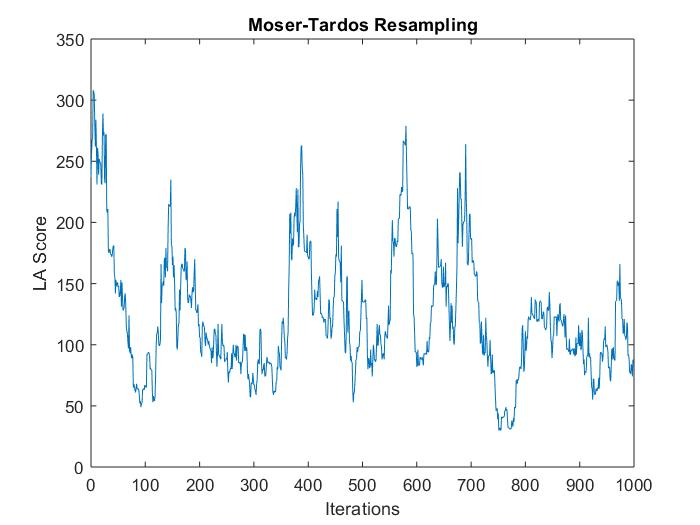
\includegraphics[width=\textwidth,keepaspectratio]{images/pure_random_construction}
\end{figure}

Therefore, in order to construct a valid locating array in this case, one would need to either increase the number of iterations or increase the number of rows in the array.
However, we also consider making a minor change to the approach itself to direct the array towards a valid solution instead of resampling purely at random.
The updated approach is discussed next.

\subsection{Directed Moser-Tardos Resampling} \label{sect:directed}

Figure \ref{fig:construction_pure_mt} shows the array score changing at random to all appearances.
In other words, some changes improve the score, while others worsen the score.
We therefore introduce a new directed construction approach that differs only slightly from Moser-Tardos resampling in that it does not accept any changes that worsen the score of the array.
After every change, the directed approach checks the array score, and if the score worsens, the change is rolled back.
It then resamples randomly repeatedly until it finds a change that does not worsen the array score.
Figure \ref{fig:construction_directed_random} shows the array score through 1000 iterations for the same construction scenario as Figure \ref{fig:construction_pure_mt}.
The score, in this case, decreases sharply and a locating array is successfully constructed after 234 iterations.
Similar to pure Moser-Tardos resampling, however, the directed resampling approach is not guaranteed to finish.

\begin{center}

\begin{figure}[htbp]
\caption{LA score after each iteration using directed Moser-Tardos resampling.}
\label{fig:construction_directed_random}
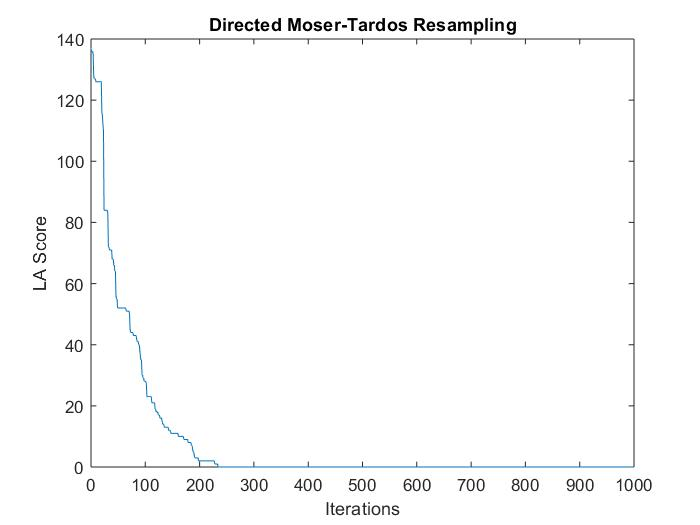
\includegraphics[width=\textwidth,keepaspectratio]{images/directed_random_construction}
\end{figure}

\end{center}

Directed Moser-Tardos resampling can also be easily modified to construct locating arrays with additional constraints such as higher separation.
Only the scoring system must be modified to indicate how close the array is to a valid locating array with a separation value $\delta$.

We modify the scoring approach described in Section \ref{sect:greedy} to score an array, $A$, with a constraint, separation $\delta$, as well.
The modified scoring approach first finds the unique pairs in the compressive sensing matrix, $M$, for $A$, where the separation requirement is violated (the violating pairs).
Then, for every violating pair, the {\em deficiency} of that pair is the number of additional row differences needed for the pair to have $\delta$ row differences.
Following the example in \cite{seidelIWOCA}, if a pair of terms $T_1$, $T_2$ exists where $T_1 \neq T_2$ but $|(\rho(A,T_1) \cup \rho(A,T_2)) \setminus ( \rho(A,T_1) \cap \rho(A,T_2))| = \mu < \delta$, then $T_1$, $T_2$ is a violating pair with deficiency $\delta-\mu$.
The score of $A$ is the same as the total deficiency of $A$ which is the sum of the deficiencies of all violating pairs.
In other words, the score counts the total additonal row differences that all violating pairs collectively need for the separation constraint to be satisfied.
Interestingly, when the only constraint for $A$ is separation $\delta = 1$, then this scoring approach is no different from the one described in Section \ref{sect:greedy}.

An interesting aspect of Algorithm \ref{alg:separation_checker} is that it is easily modified to score the locating array as well as check its validity.
When the fourth terminating condition of the algorithm is satisfied, then the number of pairs with one column in $\mathit{nodeA}$ and the other in $\mathit{nodeB}$ is multiplied by the remaining separation needed, $\delta$.
This is then added to a global variable with the total score which is initialized to zero before the initial call to the checker.
When all recursive calls are completed, the global variable holds the correct total score for a locating array with any separation constraint $\delta$.
Furthermore, this scoring change is implemented with almost no additional runtime cost.

Table \ref{tab:sizes_random} shows factor and level inputs in the first column, and the separation requirements in the second row.
The remainder of the table indicates the size, in terms of rows, needed for directed Moser-Tardos resampling to construct a valid locating array within 1000 iterations, satisfying the separation requirement.

\begin{center}

\begin{table}[htbp]
\caption{Locating array sizes using directed Moser-Tardos resampling.}
\label{tab:sizes_random}
\begin{tabularx}{\textwidth}{|2|2|2|2|2|}
\hline
& \multicolumn{4}{|c|}{Number of Rows} \\
\hline
Type & $\delta=1$ & $\delta=2$ & $\delta=3$ & $\delta=4$ \\
\hline
$2^{10}$        & 14  & 19  & 24  & 30  \\
$2^{15}$        & 17  & 22  & 29  & 34  \\
$2^{20}$        & 19  & 26  & 31  & 37  \\
$2^{50}$        & 26  & 33  & 40  & 47  \\
$2^{75}$        & 28  & 36  & 44  & 50  \\
$2^{100}$       & 31  & 39  & 46  & 53  \\
\hline
$3^{10}$        & 34  & 46  & 57  & 66  \\
$3^{15}$        & 40  & 52  & 65  & 73  \\
$3^{20}$        & 44  & 57  & 69  & 79  \\
$3^{50}$        & 57  & 70  & 83  & 95  \\
$3^{75}$        & 62  & 76  & 90  & 103 \\
$3^{100}$       & 67  & 81  & 94  & 107 \\
\hline
$4^{10}$        & 65  & 86  & 104 & 122 \\
$4^{15}$        & 76  & 96  & 116 & 133 \\
$4^{20}$        & 82  & 104 & 122 & 141 \\
$4^{50}$        & 106 & 129 & 148 & 168 \\
$4^{75}$        & 116 & 138 & 159 & 179 \\
$4^{100}$       & 123 & 146 & 166 & 188 \\
\hline
$5^{10}$        & 110 & 141 & 165 & 194 \\
$5^{15}$        & 126 & 156 & 185 & 212 \\
$5^{20}$        & 138 & 169 & 198 & 225 \\
$5^{50}$        & 173 & 208 & 236 &     \\
$5^{75}$        & 189 & 223 & 256 &     \\
$5^{100}$       & 202 & 235 & 266 &     \\
\hline
$5^{10}2^{10}$  & 110 & 139 & 172 & 197 \\
\hline
\end{tabularx}
\end{table}

\end{center}

Table \ref{tab:sizes_random} was generated using a binary search technique on the locating array size.
We began with an upper bound on the number of rows in the array that easily satisfied all constraints, and a lower bound, an empty array with 0 rows.
A binary search technique was then used to find the smallest possible size for a locating array to be constructed in 1000 iterations under the specified constraints.
In the column under $\delta = 4$, some of the cells are blank because the checker took an extended amount of time in these cases.
Not surprisingly, the locating arrays in Table \ref{tab:sizes_random} with separation $\delta = 1$ produced by directed Moser-Tardos resampling are larger than those shown in Table \ref{tab:sizes_greedy} and produced by Algorithm \ref{alg:greedy_construction} which chooses every row carefully to minimize the array score, and ultimately the final array size.

\section{Summary}

The initial greedy approach presented in Algorithm \ref{alg:greedy_construction} is convenient for creating arrays that satisfy the locating property.
It adds rows as needed, and the only necessary input parameter is factor information.
However, it is unable to construct locating arrays with additional constraints including higher separation.
Instead of modifying Algorithm \ref{alg:greedy_construction} to incorporate separation, we present randomized approaches that can be applied to construct locating arrays with any additional constraints.

Moser-Tardos resampling given in Algorithm \ref{alg:mt_construction} constructs locating arrays with additional constraints.
The main requisite of the algorithm is an efficient checker used repeatedly to check if the array satisfies all requirements.
Additionally, the algorithm requires an input parameter indicating the size of the locating array.

A modification to Moser-Tardos resampling is directed Moser-Tardos resampling discussed in Section \ref{sect:directed}.
As shown in Figure \ref{fig:construction_pure_mt} and Figure \ref{fig:construction_directed_random}, directed Moser-Tardos resampling may construct a locating array in fewer iterations than Moser-Tardos resampling.
However, it requires an additional scoring system to indicate how close the array is to satisfying all requirements.
Finally, we provide Table \ref{tab:sizes_random} to indicate the approximate locating array sizes for several different array types and separation constraints.
